\documentclass[11pt,a4paper]{article}

\usepackage{tikz}
\usetikzlibrary{nfold}
\usetikzlibrary{intersections}
\usetikzlibrary{cd}
% for zigzag decoration
\usetikzlibrary{decorations.pathmorphing}


\begin{document}

\section{pgf integration}

\subsection{nfold path and nodes with \texttt{draw}}

This used to be an issue and is the reason why \texttt{/tikz/nfold} redefines \verb"\tikz@double@setup" instead of modifying \verb"\pgf@nfold@order" directly:\\
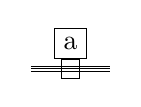
\begin{tikzpicture}
  \draw[double equal sign distance, nfold=3] (0, 0) -- (1,0) node[midway, draw, label={[draw]a}] {};
\end{tikzpicture}\\
If \texttt{/tikz/nfold} were to set \verb"\pgf@nfold@order" directly, TikZ would attempt to render the boundary of the nodes with \texttt{nfold} enabled, which results in an error.


\subsection{Saving and offsetting a soft path}

\subsubsection{Using \textbackslash pgfoffsetpath}
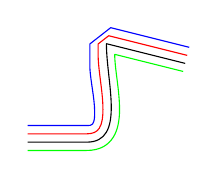
\begin{tikzpicture}[line join=bevel]
  \path[save path=\savedpath] (0,0) -- (.75,0) to[out=0, in=-90] (1,1.25) -- (2,1);
  \pgfoffsetpath{\savedpath}{0pt}
  \color{black}
  \pgfusepathqstroke
  \pgfoffsetpath{\savedpath}{3pt}
  \color{red}
  \pgfusepathqstroke
  \pgfoffsetpath{\savedpath}{6pt}
  \color{blue}
  \pgfusepathqstroke
  \pgfoffsetpath{\savedpath}{-3pt}
  \color{green}
  \pgfusepathqstroke
\end{tikzpicture}

\subsubsection{Using methods that scale correctly}
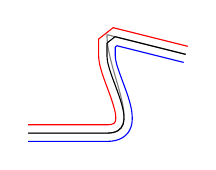
\begin{tikzpicture}[line join=bevel]
  \path[draw=gray, save path=\savedpath] (0,0) -- (1,0) to[out=0, in=-90] (1,1.25) -- (2,1);
  % Note how the path offset by 0 differs from the original path
  \pgfoffsetpathfraction{\savedpath}{6pt}{0}
  \color{black}
  \pgfusepathqstroke
  \pgfoffsetpathqfraction{\savedpath}{6pt}{.5}
  \color{red}
  \pgfusepathqstroke
  \pgfoffsetpathindex{\savedpath}{6pt}{2}{5}
  \color{blue}
  \pgfusepathqstroke
\end{tikzpicture}

\subsection{Support for pgf rectangles}
Note that this is \emph{not} called by TikZ' \texttt{rectangle} option.

\begin{pgfpicture}
  \pgfpathmoveto{\pgfpoint{-1cm}{-1cm}}
  \pgfpathlineto{\pgfpoint{1cm}{-1cm}}
  \pgfpathrectangle{\pgfpointorigin}{\pgfpoint{20pt}{20pt}}
  \pgfpathlineto{\pgfpoint{-1cm}{0cm}}
  \pgfsetlinewidth{3pt}
  \pgfsetinnerlinewidth{2pt}
  \pgfusepath{stroke,nfold}
\end{pgfpicture}

\subsection{A path without a moveto (slight bug at the moment)}
Compare
\begin{pgfpicture}
  \pgfpathlineto{\pgfpoint{1cm}{1cm}}
  \pgfpathlineto{\pgfpoint{2cm}{0cm}}
  \pgfsetlinewidth{3pt}
  \pgfsetinnerlinewidth{2pt}
  \pgfusepath{stroke}
\end{pgfpicture}
to
\begin{pgfpicture}
  \pgfpathlineto{\pgfpoint{1cm}{1cm}}
  \pgfpathlineto{\pgfpoint{2cm}{0cm}}
  \pgfsetlinewidth{3pt}
  \pgfsetinnerlinewidth{2pt}
  \pgfusepath{stroke,nfold}
\end{pgfpicture}

\subsection{An example where \textbackslash pgf@prepare@start@of@path is not called}
Here the nfold preparation code must be injected into \verb|\pgf@path@check@proper|.
{
\makeatletter
\def\pgf@prepare@start@of@path{\pgferror{not called}}
\makeatother
\begin{pgfpicture}
  \pgfpathmoveto{\pgfpointorigin}
  \pgfpathlineto{\pgfpoint{1cm}{0cm}}
  % make the path non-proper by adding a dead moveto
  \pgfpathmoveto{\pgfpointorigin}
  \pgfsetlinewidth{.3cm}
  \pgfsetinnerlinewidth{.25cm}
  \pgfsetarrows{<->}
  \pgfusepath{stroke,tips/proper,nfold=3} % likely means "only draw tips on proper arrows"
\end{pgfpicture}
}


\section{Paths and features}

\subsection{Miter limit}

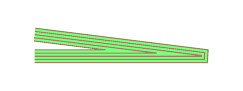
\begin{tikzpicture}[line join=miter, miter limit=16, x={(1.1cm,0)}, y={(0,1.1cm)}]
  \path[draw=green,opacity=0.5, line width=5pt] (0,0) -- (2,0) -- (0,0.25);
  \path[draw=purple, opacity=0.5, double distance=4.2pt, nfold=5] (0,0) -- (2,0) -- (0,0.25);
\end{tikzpicture}
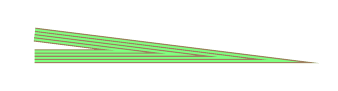
\begin{tikzpicture}[line join=miter, miter limit=17, x={(1.1cm,0)}, y={(0,1.1cm)}]
  \path[draw=green,opacity=0.5, line width=5pt] (0,0) -- (2,0) -- (0,0.25);
  \path[draw=purple, opacity=0.5, double distance=4.2pt, nfold=5] (0,0) -- (2,0) -- (0,0.25);
\end{tikzpicture}

\subsection{Angle too sharp}
{
  \makeatletter
  \def\clearerrormsg{\let\errormsg\pgfutil@empty}
  \renewcommand{\pgfutil@packagewarning}[2]{
    \ifx\errormsg\pgfutil@empty
      \xdef\errormsg{#2}
    \else
      \xdef\errormsg{\errormsg; #2}
    \fi
  }
  \makeatother

  \subsubsection{Almost 180 degree turn}
  \clearerrormsg
  
\begin{tikzpicture}
    \path[draw=purple, opacity=0.5, double distance=4.2pt, nfold] (0,0) -- (2,0) -- (0,0.01);
  \end{tikzpicture}\\
  Expectation: Finite-sized output, pgf warning ``angle too sharp''\\[.5em]
  Actual warning: \errormsg

  \subsubsection{Exactly 180 degree turn}
  \clearerrormsg
  
\begin{tikzpicture}
    \path[draw=purple, opacity=0.5, double distance=4.2pt, nfold] (0,0) -- (2,0) -- (0,0);
  \end{tikzpicture}\\
  Expectation: Finite-sized output, pgf warning ``angle too sharp''\\[.5em]
  Actual warning: \errormsg
}

\subsection{Transformed axes with relative and absolute coordinates}

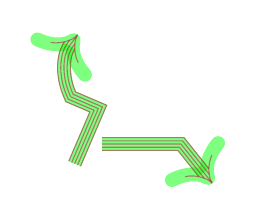
\begin{tikzpicture}[x={(.3cm,.7cm)}, y={(.7cm,-.3cm)}]
  \path[draw=green,opacity=0.5, line width=5pt, arrows=->] (1.5,1.0) -- (2.5,1.0) -- (2.5,0.5)  to[relative, out=30, in=150] (3.5,0.2);
  \path[draw=purple, opacity=0.5, arrows=-Implies, double distance=4.2pt, nfold=5]
      (1.5,1.0) -- (2.5,1.0) -- (2.5,0.5) to[relative, out=30, in=150] (3.5,0.2);
  \path[draw=green,opacity=0.5, line width=5pt, arrows=->] (1.5cm,1.0cm) -- (2.5cm,1.0cm) -- (2.9cm,0.5cm);
  \path[draw=purple, opacity=0.5, arrows=-Implies, double distance=4.2pt, nfold=5] (1.5cm,1.0cm) -- (2.5cm,1.0cm) -- (2.9cm,0.5cm);
\end{tikzpicture}

\subsection{Path with jump and cycle}
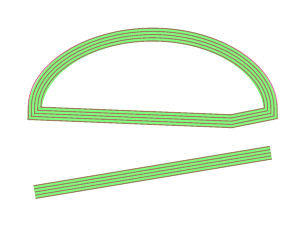
\begin{tikzpicture}
    \path [draw=green,opacity=0.5, line width=5pt] (0,0) -- (3,0.5) (3,1) arc (0:180:1.5 and 1) -- (2.5,0.9) -- cycle;
  \path[draw=purple, opacity=0.5, double distance=4.2pt, nfold=5] (0,0) -- (3,0.5) (3,1) arc (0:180:1.5 and 1) -- (2.5,0.9) -- cycle;
\end{tikzpicture}

\subsection{Multiple closed paths}
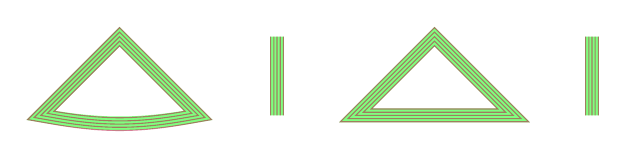
\begin{tikzpicture}
  \path [draw=green,opacity=0.5, line width=5pt, save path=\tmppath]
    (0,0) to[out=-10,in=190] (2,0) -- (1,1) -- cycle (3,0) -- (3,1)
    (4,0) -- (6,0) -- (5,1) -- cycle (7,0) -- (7,1);
  \path[draw=purple, opacity=0.5, double distance=4.2pt, nfold=5, use path=\tmppath];
\end{tikzpicture}

\subsection{Different joins in the same diagram}

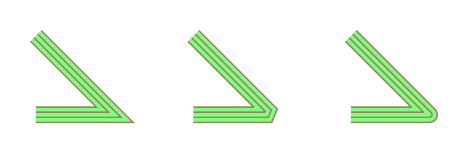
\begin{tikzpicture}[line join=bevel, double distance=5pt, line width=.5pt, draw=purple, opacity=0.5]
  \path[line join=miter, draw=green, line width=6pt] (0,0) -- (1, 0) -- (0,1);
  \path[draw=green, line width=6pt] (2,0) -- (3, 0) -- (2,1);
  \path[line join=round, draw=green, line width=6pt] (4,0) -- (5, 0) -- (4, 1);
  \path[draw, line join=miter, double distance=5pt, nfold=4] (0,0) -- (1, 0) -- (0,1);
  \path[draw, double distance=5pt, nfold=4] (2,0) -- (3, 0) -- (2,1);
  \path[draw, line join=round, double distance=5pt, nfold=4] (4,0) -- (5, 0) -- (4, 1);
\end{tikzpicture}

\subsection{Shorten}
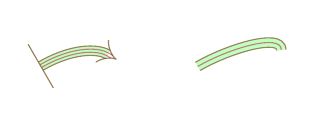
\begin{tikzpicture}
  \draw[draw=green,opacity=.5,double distance=3pt, shorten >= 3pt, shorten <=-2pt, arrows=|-Implies] (0,0) to[bend left] (1,0);
  \draw[draw=purple, opacity=.5,double distance=3pt, shorten >= 3pt, shorten <=-2pt, arrows=|-Implies, nfold=4] (0,0) to[bend left] (1,0);
  \draw[draw=green,opacity=.5,double distance=3pt, shorten >= 5pt, shorten <=-2pt] (2,0) to[out=30,in=90] (3,0);
  \draw[draw=purple, opacity=.5, double distance=3pt, shorten >= 5pt, shorten <=-2pt, nfold=3] (2,0) to[out=30,in=90] (3,0);
\end{tikzpicture}

\subsection{Different types of tips}
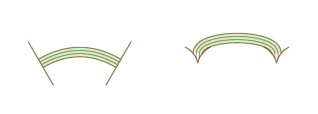
\begin{tikzpicture}
  \draw[draw=green,opacity=.5,double distance=3pt, arrows=|-|] (0,0) to[bend left] (1,0);
  \draw[draw=purple, opacity=.5,double distance=3pt, arrows=|-|, nfold=4] (0,0) to[bend left] (1,0);
  \draw[draw=green,opacity=.5,double distance=3pt, arrows=Implies-Implies] (2,0) to[out=90,in=90] (3,0);
  \draw[draw=purple, opacity=.5, double distance=3pt, nfold=4, arrows=Implies-Implies] (2,0) to[out=90,in=90] (3,0);
\end{tikzpicture}

\subsection{More extreme paths}
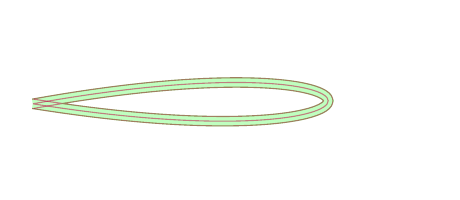
\begin{tikzpicture}
  \draw[draw=green,opacity=.5,double distance=3pt] (0,0) .. controls (5,.9) and (5,-.8) .. (0,0);
  \draw[draw=purple, opacity=.5,double distance=3pt, nfold=3] (0,0) .. controls (5,.9) and (5,-.8) .. (0,0);
\end{tikzpicture}
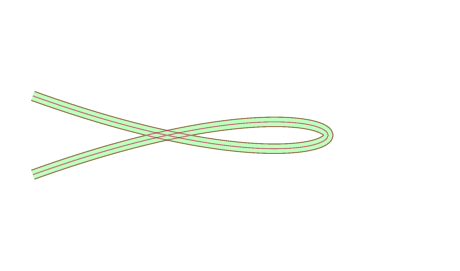
\begin{tikzpicture}
  \draw[draw=green,opacity=.5,double distance=3pt] (0,-.5) .. controls (5, 1.3) and (5,-1.3) .. (0,.5);
  \draw[draw=purple, opacity=.5,double distance=3pt, nfold=3] (0,-.5) .. controls (5, 1.3) and (5,-1.3) .. (0,.5);
\end{tikzpicture}

\subsection{Degenerate paths and tips}

\begin{tikzpicture}
  \draw[draw=green,opacity=.5,double distance=3pt, arrows=|-|] (0,0) (.25,0) -- (.75,0) (1,0);
  \draw[draw=purple, opacity=.5,double distance=3pt, arrows=|-|, nfold=4] (0,0) (.25,0) -- (.75,0) (1,0);
  \draw[draw=green,opacity=.5,double distance=3pt, arrows=Implies-Implies] (2,0) (2.25,0) -- (2.75,0) (3,0);
  \draw[draw=purple, opacity=.5, double distance=3pt, nfold=4, arrows=Implies-Implies] (2,0) (2.25,0) -- (2.75,0) (3,0);
\end{tikzpicture}


\subsection{Dashed}

\begin{tikzpicture}
  \draw[arrows=-Implies, double equal sign distance, dashed, nfold] (0,0) -- (1,0);
  \draw[arrows=-Implies, double equal sign distance, dashed, nfold] (2,0) to[out=30, in=150] (4,0);
\end{tikzpicture}\\
The desynchronisation in the latter case is a fundamental limitation of this approach.


\subsection{Short straight lines and large angles}

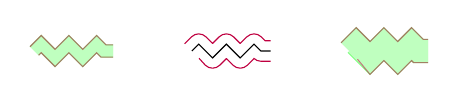
\begin{tikzpicture}
  \draw[green, double distance=4pt, decorate, decoration=zigzag, opacity=.5] (0,0) -- (1,0);
  \draw[purple, double distance=4pt, decorate, decoration=zigzag, nfold, opacity=.5] (0,0) -- (1,0);
  \draw[black,decorate, decoration=zigzag] (2,0) -- (3,0);
  \draw[purple, double distance=7pt, decorate, decoration=zigzag, nfold, line join=round] (2,0) -- (3,0);
  \draw[green, double distance=8pt, decorate, decoration=zigzag, opacity=.5] (4,0) -- (5,0);
  \draw[purple, double distance=8pt, decorate, decoration=zigzag, nfold, opacity=.5] (4,0) -- (5,0);
\end{tikzpicture}
\vspace{1cm}

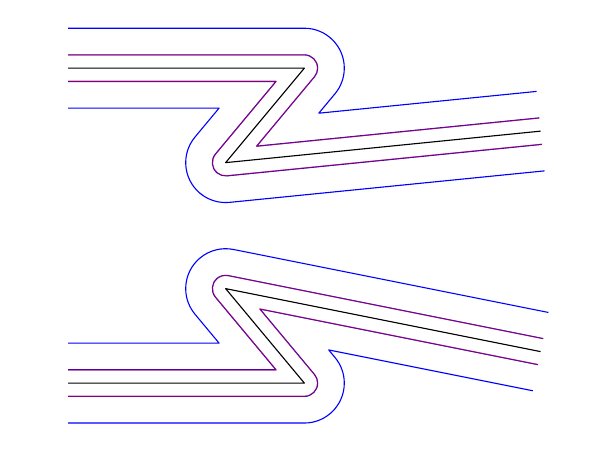
\begin{tikzpicture}[line join=round]
  \draw[black] (0, 0) -- (3,0) -- (2, 1.2) -- (6, .4);
  \draw[blue, double distance=1cm, nfold=4] (0, 0) -- (3,0) -- (2, 1.2) -- (6, .4);
  \draw[red, double distance=.32cm, nfold=2, opacity=.5] (0, 0) -- (3,0) -- (2, 1.2) -- (6, .4);
  \draw[black] (0, 4) -- (3,4) -- (2, 4-1.2) -- (6, 4-.8);
  \draw[blue, double distance=1cm, nfold=4] (0, 4) -- (3,4) -- (2, 4-1.2) -- (6, 4-.8);
  \draw[red, double distance=.32cm, nfold=2, opacity=.5] (0, 4) -- (3,4) -- (2, 4-1.2) -- (6, 4-.8);
\end{tikzpicture}

\subsection{Closed paths and the close joins edge case}
\subsubsection{Short first segment}
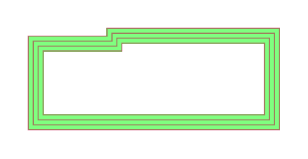
\begin{tikzpicture}
  \draw[draw=green,opacity=0.5, line width=5.8pt, save path=\tmppath] (1,1) -- (1,1.1) -- (3,1.1) -- (3,0) -- (0,0) -- (0,1) -- cycle;
  \path[draw=purple, opacity=0.5, double distance=5pt, nfold=4, use path=\tmppath];
\end{tikzpicture}

\subsubsection{Short last segment}
This edge case needs special handling which is not implemented yet.\\
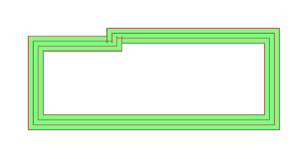
\begin{tikzpicture}
  \draw[draw=green,opacity=0.5, line width=5.8pt, save path=\tmppath] (1,1.1) -- (3,1.1) -- (3,0) -- (0,0) -- (0,1) -- (1,1) -- cycle;
  \path[draw=purple, opacity=0.5, double distance=5pt, nfold=4, use path=\tmppath];
\end{tikzpicture}

\subsection{Key \texttt{/tikz/scaling nfold}}

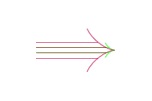
\begin{tikzpicture}
  % wrong way round disables scaling
  \draw[double equal sign distance, nfold, arrows=-Implies, green, opacity=.5] (0,0) -- (1,0);
  \draw[double equal sign distance, scaling nfold=4, arrows=-Implies, purple, opacity=.5] (0,0) -- (1,0);
\end{tikzpicture}

\subsection{Singular and almost singular curves}

\subsubsection{Exactly singular}

\begin{tikzpicture}
  \draw[double distance=5pt, nfold] (.5,1) -- (1,0) .. controls (1,0) and (1.1, 1) .. (2,1);
  \draw[red] (.5,1) -- (1,0) .. controls (1,0) and (1,1) .. (2,1);
  \draw[double distance=5pt, nfold] (4,1) .. controls (3.1,1) and (3,0) .. (3,0) --  (2.5,1);
\end{tikzpicture}

\subsubsection{Almost singular}
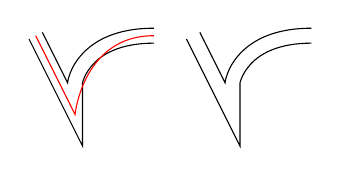
\begin{tikzpicture}
  \draw[double distance=5pt, nfold] (.5,1) -- (1,0) .. controls (1,.1) and (1.1,1) .. (2,1);
  \draw[red] (.5,1) -- (1,0) .. controls (1,0) and (1.1,1) .. (2,1);
  \draw[double distance=5pt, nfold] (4,1) .. controls (3.1,1) and (3,.1) .. (3,0) --  (2.5,1);
\end{tikzpicture}\\
Both the larger discrepancy between the red line and the double path and the slight corner at the join are expected.

\section{Checking for undesired global effects}

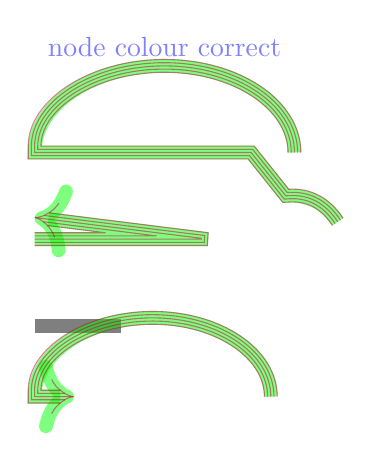
\begin{tikzpicture}[line join=miter, miter limit=10, x={(1.1cm,0)}, y={(0,1.1cm)}]
  \path [draw=green,opacity=0.5, line width=5pt, arrows=->] (3,1) arc (0:180:1.5 and 1) -- (0.5,1.0) -- (2.5,1.0) -- (2.9,0.5)  to[relative, out=30, in=150] (3.5,0.2) (0,0) -- (2,0) -- (0,0.25) ;
  \path[draw=purple, opacity=0.5, arrows=-Implies, double distance=4.2pt, nfold=5]
    (3,1) arc (0:180:1.5 and 1) node[blue, midway, above] {node colour correct} -- (0.5,1.0) -- (2.5,1.0) -- (2.9,0.5) to[relative, out=30, in=150] (3.5,0.2)
  (0,0) -- (2,0) -- (0,0.25);
  % make sure the subsequent path is unaffected
  \draw[line width=5pt, opacity=.5] (0,-1)  -- (1, -1);
    \path[draw=green,opacity=0.5, line width=5pt, arrows=->]
    (3 cm,-2 cm) arc (0:180:1.5 cm and 1 cm) -- (0.5 cm,-2 cm);
    \path
    [draw=purple,opacity=0.5, arrows=-Implies, double distance=4.2pt, nfold=5]
    (3 cm,-2 cm) arc (0:180:1.5 cm and 1 cm) -- (0.5 cm,-2 cm);
\end{tikzpicture}

\section{tikz-cd compatibility}

\begin{tikzcd}[row sep=1.5cm]
      a_2 \ar[d, Rightarrow, double distance=10pt, nfold]
    & a_3 \ar[d, Rightarrow, double distance=10pt, nfold=3]
    & a_4 \ar[d, Rightarrow, double distance=10pt, nfold=4]
    & a_5 \ar[d, Rightarrow, double distance=10pt, nfold=5]
    & a_6 \ar[d, Rightarrow, double distance=10pt, nfold=6]
    & a_7 \ar[d, Rightarrow, double distance=10pt, nfold=7]
    \\
  b_2 \ar[r, Mapsto, color=green, opacity=.5]  \ar[r, Mapsto, nfold, purple, opacity=.5] & b_3 \ar[r, Mapsto, double distance=3pt, nfold=3] & b_4 \ar[r, Mapsfrom, nfold=3] & b_5 & b_6 & b_7
\end{tikzcd}

\subsection{Scaling test}

\begin{tikzcd}[row sep=1.5cm]
      a_2 \ar[d, Rightarrow, scaling nfold, "b", "a"']
      \ar[d, purple, opacity=.5, Rightarrow, "b", "a"']
    & a_3 \ar[d, Rightarrow, scaling nfold=3, "b", "a"']
    & a_4 \ar[d, Rightarrow, scaling nfold=4, "b", "a"']
      \ar[d, purple, opacity=.5, Rightarrow, nfold]
    & a_5 \ar[d, Rightarrow, scaling nfold=5, "b", "a"']
    & a_6 \ar[d, Rightarrow, scaling nfold=6, "b", "a"']
      \ar[d, purple, opacity=.5, Rightarrow, nfold]
    & a_7 \ar[d, Rightarrow, scaling nfold=7, "b", "a"'] \\
  b_2 \ar[r, Mapsto, color=green, opacity=.5]  \ar[r, Mapsto, nfold, purple, opacity=.5] & b_3 \ar[r, Mapsto, double distance=3pt, nfold=3] & b_4 \ar[r, Mapsfrom, nfold=3] & b_5 & b_6 & b_7
\end{tikzcd}


\subsection{Testing compatibility with various features}

\newcommand{\testarrow}[2]{
  \def\testoptions##1{[##1]}
  \expandafter\ar\testoptions{Rightarrow,red,opacity=.8,#1}
  \expandafter\ar\testoptions{Rightarrow,opacity=.7,green!70!black,#1,#2}
}
\begin{tikzcd}[scale=1.1]
  a_1
  \testarrow{dr, shift left=-10pt, shorten <=5pt, shorten >=3pt,
    out=-10, in=110, "l", "m"'}{nfold=3}
  & a_2
  \testarrow{%
    d,double distance between line centers=5pt, "a" inner sep=3.5pt,
    "o"' inner sep=3.5pt, shorten >=-5pt, shorten <=-1pt, bend left=30
  }{nfold=5}
  \\
  b_1 & b_2 \\
  c_1
  \testarrow{d,"a", "b"', bend left=30}{nfold}
  \testarrow{r}{nfold}
  & c_2 
  \testarrow{dr,shift left=-1pt, out=30, in=180,"l", "m"'}{nfold}
  & c_3 \\
  d_1 \testarrow{r, bend right, double distance=5pt, "a","b"'}{nfold=5} & d_2 & d_3
\end{tikzcd}

\subsection{Squiggly (issue \#4)}

\begin{tikzcd}
  \bullet & \bullet
  \arrow[Rightarrow, squiggly, from=1-1, to=1-2, green]
  \arrow[Rightarrow, squiggly, from=1-1, to=1-2, nfold, purple, opacity=.5]
\end{tikzcd}

\end{document}
